\section{Физическая модель маятника}

Рассмотрим систему, состоящую из тележки массой $M$, движущейся по горизонтальной оси, и маятника с равномерно распределенной массой $m$ и длиной $l_{\text{pend}}$,
закрепленного на шарнире на тележке. Примем за $x$ координату тележки, а за $\theta$ угол отклонения маятника от вертикали. Схема системы представлена на рисунке \ref{fig:pendulum}.
\begin{figure}[ht!]
    \centering
    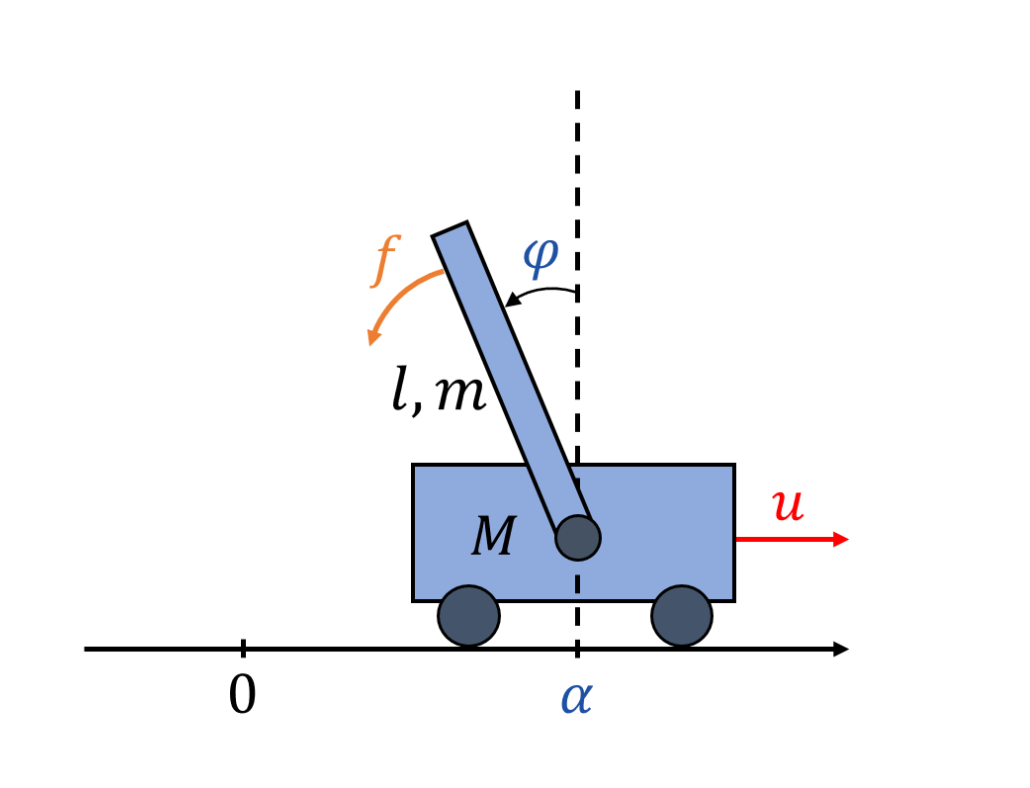
\includegraphics[width=0.5\textwidth]{media/cart.png}
    \caption{Схема маятника на тележке}
    \label{fig:pendulum}
\end{figure}

\subsection{Уравнения движения}
Используем законы Лагранжа для записи уравнений движения системы. 

Так как кинетическая и потенциальная зависят от центра масс тележки и маятника, введем в рассмотрение расстояние $l$ 
от точки подвеса маятника до его центра масс. При этом $l = l_{\text{pend}}/2$ для равномерно распределенной массы маятника.

Напишем уравнения для координат центра масс маятника $x_m$ и $y_m$ и продифференцировав их по времени, получим скорости центра масс маятника:
\begin{equation}
    \begin{cases}
        x_m = x + l\sin\theta, \\
        y_m = l\cos\theta
    \end{cases} \Rightarrow
    \begin{cases}
        v_x = \dot{x} + l\dot{\theta}\cos\theta, \\
        v_y = -l\dot{\theta}\sin\theta
    \end{cases}
\end{equation}
Общая энергия системы складывается из кинетической и потенциальной энергии маятника и кинетической энергии тележки:

Кинетическая энергия системы равна:
\begin{equation}
    T = \frac{1}{2} (M + m)\dot{x}^2 + m\dot{x}l\dot{\theta}\cos\theta + \frac{1}{2}ml^2\dot{\theta}^2
\end{equation}
Потенциальная энергия системы равна:
\begin{equation}
    U = mgl\cos\theta
\end{equation}
Записывая функция Лагранжа $L = T - U$, получаем: 
\begin{equation}
    L = \frac{1}{2} (M + m)\dot{x}^2 + m\dot{x}l\dot{\theta}\cos\theta + \frac{1}{2}ml^2\dot{\theta}^2 - mgl\cos\theta
\end{equation}
Уравнения Лагранжа примут вид:
\begin{equation}
    \begin{array}{cc}
        \frac{d}{dt} \left( \frac{\partial L}{\partial \dot{x}} \right) - \frac{\partial L}{\partial x} = Q_x, \\
        \frac{d}{dt} \left( \frac{\partial L}{\partial \dot{\theta}} \right) - \frac{\partial L}{\partial \theta} = Q_{\theta}
    \end{array}
\end{equation}
где $Q_x$ и $Q_{\theta}$ -- обобщенные силы, действующие на тележку и маятник соответственно. В итоге получаем систему уравнений:
\begin{equation}
    \begin{cases}
        (M + m)\ddot{x} + ml\ddot{\theta}\cos\theta - ml\dot{\theta}^2\sin\theta = Q_x, \\
        ml^2\ddot{\theta} + ml\ddot{x}\cos\theta - mgl\sin\theta = Q_{\theta}.
    \end{cases}
    \label{eq:forces_balance}
\end{equation}
Система уравнений \eqref{eq:forces_balance} представляет собой уравнения баланса сил, 
приложенных к тележке и моментов, действующих на маятник.

Запишем этм уравнения разрешив их относительно высших производных. Заметим, что вторые производные 
входят в эти уравнения линейно. С учетом этого приведем уравнения к матричному виду:  % # TODO: analiz_ustoychivosti_perevernutogo_mayatnika_v_srede_matlab_control
\begin{equation}
    \begin{bmatrix}
        ml^2 & ml\cos\theta \\
        ml\cos\theta & M + m \\
    \end{bmatrix} \times
    \begin{bmatrix}
        \ddot{\theta} \\
        \ddot{x} \\
    \end{bmatrix} =
    \begin{bmatrix}
        mgl\sin\theta + Q_{\theta} \\
        ml\dot{\theta}^2\sin\theta + Q_x
    \end{bmatrix}
\end{equation}
Убедимся в существовании и единственности решения системы:
\begin{equation}
    D = ml^2(M + m) - m^2l^2\cos^2\theta = ml^2(M + m - m\cos^2\theta) > 0
\end{equation}
Решая систему уравнений методом Крамера, получаем:
\begin{multline}
    \Delta_{\ddot{\theta}} = \begin{vmatrix}
        mgl\sin\theta + Q_{\theta} & ml\cos\theta \\
        ml\dot{\theta}^2\sin\theta + Q_x & M + m \\
    \end{vmatrix} = (mgl\sin\theta + Q_{\theta})(M + m) - ml\cos\theta(ml\dot{\theta}^2\sin\theta + Q_x) 
\end{multline}
\begin{multline}
    \Delta_{\ddot{x}} = \begin{vmatrix}
        ml^2 & mgl\sin\theta + Q_{\theta} \\
        ml\cos\theta & ml\dot{\theta}^2\sin\theta + Q_x \\
    \end{vmatrix} = ml^2(ml\dot{\theta}^2\sin\theta + Q_x) - ml\cos\theta(mgl\sin\theta + Q_{\theta})
\end{multline}

\begin{equation}
    \begin{cases}
        \ddot{x} = \frac{ml^2(ml\dot{\theta}^2\sin\theta + Q_x) - ml\cos\theta(mgl\sin\theta + Q_{\theta})}{ml^2(M + m - m\cos^2\theta)} \\ 
        \ddot{\theta} = \frac{(mgl\sin\theta + Q_{\theta})(M + m) - ml\cos\theta(ml\dot{\theta}^2\sin\theta + Q_x)}{ml^2(M + m - m\cos^2\theta)} \\ 
    \end{cases}
    \label{eq:nonlinear_model}
\end{equation}

Можно записать систему в пространстве состояний $X$ в форме Коши: 
\begin{equation}
    \begin{array}{cc}
        X = \begin{bmatrix} 
            x \\
            \dot{x} \\
            \theta \\
            \dot{\theta}
    \end{bmatrix} & 
    \dot{X} = \begin{bmatrix}
        \dot{x} \\
        \frac{ml^2(ml\dot{\theta}^2\sin\theta + Q_x) - ml\cos\theta(mgl\sin\theta + Q_{\theta})}{ml^2(M + m - m\cos^2\theta)}
        \dot{\theta} \\
        \frac{(mgl\sin\theta + Q_{\theta})(M + m) - ml\cos\theta(ml\dot{\theta}^2\sin\theta + Q_x)}{ml^2(M + m - m\cos^2\theta)} \\ 
    \end{bmatrix}
    \end{array}
\end{equation}
Измеряемым выходом системы будет считать вектор $Y$, состоящий из координат тележки и угла отклонения маятника от вертикали:
\begin{equation}
    Y = \begin{bmatrix}
        1 & 0 & 0 & 0 \\
        0 & 0 & 1 & 0 \\ 
    \end{bmatrix} X
\end{equation}

\subsection{Точки равновесия}
Найдем точки равновесия системы в отсутствие внешних сил ($Q_x = Q_{\theta} = 0$). 
Для этого приравняем к нулю правые части уравнений движения, решим систему уравнений:
\begin{equation}
    \dot{X} = 0 \Rightarrow 
    \begin{cases}
        \dot{x} = 0, \\
        \dot{\theta} = 0, \\
        \frac{(mgl\sin\theta + Q_{\theta})(M + m) - ml\cos\theta(ml\dot{\theta}^2\sin\theta + Q_x)}{ml^2(M + m - m\cos^2\theta)} = 0 \\ 
        \frac{ml^2(ml\dot{\theta}^2\sin\theta + Q_x) - ml\cos\theta(mgl\sin\theta + Q_{\theta})}{ml^2(M + m - m\cos^2\theta)} = 0
    \end{cases}
\end{equation}
Упростив, получаем: 
\begin{equation}
    \begin{cases}
        \sin\theta(g(M + m) - \cos\theta(ml)) = 0 \\ 
        \sin\theta(ml - \cos\theta g) = 0
    \end{cases}
\end{equation}
Решая систему уравнений, получаем:
\begin{equation}
    \sin\theta = 0 \Rightarrow \theta = 0, \pi 
\end{equation}
Таким образом, точки равновесия системы определяются углом отклонения маятника от вертикали $\theta = 0$ и $\theta = \pi$, 
что соответствует наивысшему и наинизшему положению маятника соответственно, что сходится с ожидаемым результатом. 

\subsection{Линейная модель}
Для дальнейшего анализа системы ее необходимо линеаризовать. Линеаризацию необходимо проводить в точках равновесия 
системы, которые были найдены в предыдущем пункте, в противном случае отклонения линейной модели от реальной системы будут велики. 
Линеаризуем систему в точке равновесия $\theta = 0$ и $x = 0$, используя то, что $\sin x \approx x$, $\cos x \approx 1$, $x^{n + 1} \approx 0, n \in N$ 
при малых $x$. 
\begin{equation}
    \dot{X} = \begin{bmatrix}
        \dot{x} \\
        \frac{lQ_x - mgl\theta - Q_{\theta}}{lM} \\
        \dot{\theta} \\
        \frac{(g\theta + Q_{\theta})(M + m) -Q_x}{lM} \\ 
    \end{bmatrix}
\end{equation}
Запишем систему в матричном виде, принимая за управление обобщенную силу, приложенную на каретку, а за внешнее 
внешнее возмущение обобщенную силу, приложенную на маятник $u = Q_x, f = Q_{\theta}$:
\begin{equation}
    \begin{cases}
        \dot{x} = Ax + Bu + Df \\ 
        y = Cx
    \end{cases}
    \label{eq:linear_model}
\end{equation}
\begin{equation}
    \begin{array}{cc}
        \begin{bmatrix}
        \dot{x} \\
        \ddot{x} \\
        \dot{\theta} \\
        \ddot{\theta} \\
    \end{bmatrix} = \begin{bmatrix}
        0 & 1 & 0 & 0 \\
        0 & 0 & \frac{-mg}{M} & 0 \\
        0 & 0 & 0 & 1 \\
        0 & 0 & \frac{g(M + m)}{lM} & 0 \\
    \end{bmatrix} \times \begin{bmatrix}
        x \\
        \dot{x} \\
        \theta \\
        \dot{\theta} \\
    \end{bmatrix} + \begin{bmatrix}
        0 \\
        \frac{1}{M} \\
        0 \\
        \frac{-1}{lM} \\
    \end{bmatrix} \times Q_x + \begin{bmatrix}
        0 \\
        \frac{-1}{lM} \\
        0 \\
        \frac{M + m}{lM} \\ 
    \end{bmatrix} \times Q_{\theta}  \\[4em]
    y = \begin{bmatrix}
        1 & 0 & 0 & 0 \\
        0 & 0 & 1 & 0 \\ 
    \end{bmatrix} \times \begin{bmatrix}
        x \\
        \dot{x} \\
        \theta \\
        \dot{\theta} \\
    \end{bmatrix}
    \end{array}
\end{equation}
Таким образом, матрицы системы примут вид: 
\begin{equation}
    A = \begin{bmatrix}
        0 & 1 & 0 & 0 \\
        0 & 0 & \frac{-mg}{M} & 0 \\
        0 & 0 & 0 & 1 \\
        0 & 0 & \frac{g(M + m)}{lM} & 0 \\
    \end{bmatrix}, B = \begin{bmatrix}
        0 \\
        \frac{1}{M} \\
        0 \\
        \frac{-1}{lM} \\
    \end{bmatrix}, D = \begin{bmatrix}
        0 \\
        \frac{-1}{lM} \\
        0 \\
        \frac{M + m}{lM} \\ 
    \end{bmatrix}, C = \begin{bmatrix}
        1 & 0 & 0 & 0 \\
        0 & 0 & 1 & 0 \\ 
    \end{bmatrix}
\end{equation}
